\documentclass{beamer}
\usepackage{amsmath,amssymb,amsfonts,amsthm}
\usepackage[latin1]{inputenc}
\usepackage[francais]{babel}
\usepackage{graphicx}
\usepackage{default}

\title{Structuring the Synthesis of Heap-Manipulating Programs}

\author{NADIA POLIKARPOVA, UCSD, USA \\ILYA SERGEY, University College London, UK}

\date{}
\begin{document}
	\maketitle
\begin{frame}[fragile]
	\frametitle{Introduction}
	
	\begin{center}
		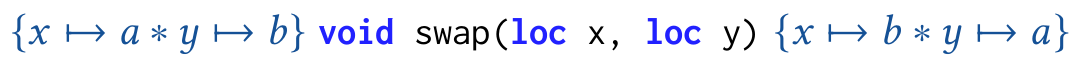
\includegraphics[height=\baselineskip]{figures/swap.png}
	\end{center}
	Motivation : Faire avancer l'�tat de l'art en mati\'ere in synthesizing provably correct
	heap-manipulating programs from declarative functional specifications
\end{frame}
\begin{frame}[fragile]
	\frametitle{Sp\'ecifications pour la Synth\`ese}
\end{frame}
\begin{frame}[fragile]
	\frametitle{R\`egles d'Inf\'erence Basiques}
\end{frame}
\begin{frame}[fragile]
	\frametitle{Unification Spatiale et Backtrack}
\end{frame}
\begin{frame}[fragile]
	\frametitle{Raisonner sur les contraintes pures}
	\framesubtitle{Pr\'econditions}
\end{frame}
\begin{frame}[fragile]
	\frametitle{Raisonner sur les contraintes pures}
	\framesubtitle{Postconditions}
\end{frame}
\begin{frame}[fragile]
	\frametitle{Synth\`ese pour pr\'edicats inductifs}
	\framesubtitle{M\'emoire dynamique}
\end{frame}
\begin{frame}[fragile]
	\frametitle{Synth\`ese pour pr\'edicats inductifs}
	\framesubtitle{Induction}
\end{frame}
\begin{frame}[fragile]
	\frametitle{Synth\`ese pour pr\'edicats inductifs}
	\framesubtitle{D\'eroulement de pr\'edicat}
\end{frame}
\begin{frame}[fragile]
	\frametitle{Synth\`ese pour pr\'edicats inductifs}
	\framesubtitle{Etiquette de niveau}
\end{frame}
\begin{frame}[fragile]
	\frametitle{Synth\`ese pour pr\'edicats inductifs}
	\framesubtitle{D\'eroulement dans la postcondition}
\end{frame}
\begin{frame}[fragile]
	\frametitle{Permettre l'appel de proc\`edure}
	\framesubtitle{Enl\'evement de l'appel}
\end{frame}
\begin{frame}[fragile]
	\frametitle{Synthetic Separation Logic}
\end{frame}
\begin{frame}[fragile]
	\frametitle{Garanties Formelles}
\end{frame}
\begin{frame}[fragile]
	\frametitle{Algorithme de synth\`ese bas\'e sur SSL}
\end{frame}
\begin{frame}[fragile]
	\frametitle{Optimisations et extensions}
	Optimisations :
	\begin{itemize}
		\item R\`egles inversibles
		\pause
		\item Recherche multi-phase
		\pause
		\item R\`eduction des sym\'etries
		\pause
		\item R\`egles d'\'echec 
	\end{itemize}
	\pause
	Extensions :
	\begin{itemize}
	\item Fonctions auxilliaire
	\pause
	\item Enl\`evement de branches	
	\end{itemize}
\end{frame}
\begin{frame}
	\frametitle{Benchmark}
\end{frame}


\end{document}
